\section{量子カオスとしてのSYK模型}

\subsection{量子重力の揺らぎ}
量子重力の大きい謎の1つは、ブラックホールのミクロな状態が持つ離散スペクトラムの起源である。
量子論が本質的に持つ離散スペクトラムの存在は、2点関数を用いる事によって調べる事ができる:
\begin{align}
	G(t)
		&= \frac{1}{Z(\beta)}\mathrm{tr}\left[e^{-\beta H}O(t)O(0)\right]\nonumber\\
		&= \frac{1}{Z(\beta)}\sum_{m, n}e^{-\beta E_m}
			|\langle m|O|n \rangle|^2e^{i(E_m - E_n)t}.
	\label{eq:twopointfunc_of_O}
\end{align}
ここで$O$はあるエルミート演算子、$Z = \mathrm{tr}(e^{-\beta H})$は分配関数、
そして$|n\rangle$は固有値$E_n$を持つエネルギーの固有状態である。
$t$が小さい時は級数を粗子化して滑らかな密度の積分に置き換える事ができ、$G(t)$は指数関数的に0に落ちる。
しかしこの振る舞いはずっと続く訳ではなく、$t$が大きい時にはスペクトラムの離散性が重要になっていき、
\eqref{eq:twopointfunc_of_O}式の波の位相によって$G(t)$は激しく振動し、もはや0には落ちない。

ホログラフィック原理において、粗子化による近似は古典重力への量子補正を加えた摂動計算と同じであり、
この近似の範疇では$G(t)$の値はずっと落ち続ける。
よって量子論の持つ離散性が見えておらず、量子重力ではそれに対する補正項の存在があるはずである。

離散スペクトラムの存在を調べるには、2点関数よりも次式のような量を用いる方が単純化される:
\begin{align}
	Z(\beta, t) = \mathrm{tr}\ e^{-\beta H - itH}.
\end{align}
これは分配関数$Z(\beta)$を$\beta\to\beta + it$のように解析接続して得られる。
$t$が大きい時では$Z(\beta, t)$は$G(t)$と同様に激しく振動する。

$t$が大きい時のある量の振る舞いを調べるには時間平均を取るという事がしばしば行われる。
$Z(\beta, t)$の時間平均はゼロであるので、$Z(\beta, t)$は大きい$t$でゼロのまわりで揺らぐという事が言える。
その揺らぎの大体のサイズは
\begin{align}
	\left|\frac{Z(\beta, t)}{Z(\beta)}\right|^2
	= \frac{1}{Z(\beta)^2}\sum_{m,n}e^{-\beta(E_m + E_n)}e^{i(E_m - E_n)t}
\end{align}
で与えられる。
一般にこの揺らぎのサイズの$t \gg 1$での振る舞いを調べるのは容易ではないが、
長時間平均を取る事によって計算がいくらか簡単になる。
長時間平均を取ると有限の位相を持つ波は全てゼロに均され、$E_n-E_m = 0$の項のみが残り次式にたどり着く:
\begin{align}
	\lim_{T\to\infty}\frac{1}{T}\int_0^Tdt\ \left|\frac{Z(\beta, t)}{Z(\beta)}\right|^2
	= \frac{1}{Z(\beta)^2}\sum_E N_E^2e^{-2\beta E}.
\end{align}
ここで$N_E$は縮退度であり、スペクトラムに縮退が存在しない i.e. $N_E = 1$であるならば
\begin{align}
	\lim_{T\to\infty}\frac{1}{T}\int_0^Tdt\ \left|\frac{Z(\beta, t)}{Z(\beta)}\right|^2
	= \frac{Z(2\beta)}{Z(\beta)^2}
	\label{eq:average_of_fluctuation_of_Z}
\end{align} 
となる。
$Z$のスケールは一般的にエントロピー$S$とある定数$a > 0$を用いて$Z \approx e^{aS}$である。
よって$Z$の揺らぎの長時間平均\eqref{eq:average_of_fluctuation_of_Z}式は大体
$e^{-aS}$という大きさを持つ。
AdS/CFT対応の文脈では$S$はブラックホールエントロピーであり、そのスケールは、
バルク理論のストリング結合定数$g_s$とニュートン定数$G_N$を用いて、$1/g_s^2 \approx 1/G_N$で与えられる。
よって\eqref{eq:average_of_fluctuation_of_Z}式はバルク理論における非摂動計算となる。
ラージブラックホールでは$S$は境界側の場の理論の熱力学的エントロピーであり、その大きさは系の自由度で
与えられる。
超対称性非可換ゲージ理論ならば$S\approx N^2$であり、SYK模型ならば$S\approx N$となる。
いずれにせよ\eqref{eq:average_of_fluctuation_of_Z}式は$1/N$の非摂動的量である。

ここで\eqref{eq:average_of_fluctuation_of_Z}式の左辺を粗子化近似によって計算しようとすると、
離散スペクトラムを走る和が滑らかな密度の積分に置き換わり、結果としてゼロとなり
\eqref{eq:average_of_fluctuation_of_Z}式の右辺と一致しない。
よって$Z$の揺らぎの大きさがゼロにならないのは何故かを探求する事で、
ブラックホールのスペクトラムの離散性や量子論を探る事ができる。
この研究において、$\mathcal{N}=4$超対称非可換ゲージ理論よりも解析が可能という理由で
SYK模型は良い"研究室"となっている。

以下では、基本的にはSYK模型における分配関数の揺らぎの大きさの平均を調べる事になる。
ただしSYK模型はランダム結合定数$J_{ijkl}$を持つので、長時間平均の代わりに$J_{ijkl}$で平均を
取る(disorder average):
\begin{align}
	g(t) \equiv
	\frac{\average{Z(\beta, t)Z(\beta, t)^*}_J}{\average{Z(\beta)^2}_J}.
	\label{eq:spectral_form_factor}
\end{align}
ここで分母と分子をまとめて平均操作を施すという選択肢もあるが、ここでは別々に分子と分母の平均を取った。
このような量を annealed quantity という。
こうするメリットとしてはレプリカの数が有限で済むという事が挙げられる。
すなわち、\eqref{eq:spectral_form_factor}式は基本的に$ZZ^*$の期待値なので、
言ってみれば$Z$に対応する系と$Z^*$のそれというようにSYKの系を2つコピーしたと言える。
もし分母と分子をまとめて平均取ったとすると、このコピーの数が任意個になってしまう。

$g(t)$は量子カオスの分野において重要なスペクトラル統計の量であり、
スペクトラル形状因子と呼ばれる
\footnote{量子カオスやスペクトラル統計の詳細は\ref{app:quantum_chaos}を参照する事。}。
スペクトラル統計ではランダム行列理論(Random Matrix Theory: RMT)という数学が用いられる。
量子カオスの分野における基本的な仮定の1つに、エネルギー固有値の統計的構造がRMT
におけるランダム行列のそれと一致するというものがある。
このランダム行列の要素が従う確率分布には3種類あり、それぞれGaussian Unitary Ensemble(GUE),
Gaussian Orthogonal Ensemble(GOE), Gaussian Symplectic Ensemble(GSE)と呼ばれる。
どれを用いるかは系の持つ対称性によって決まる。
RMTは基本的に複数の固有値の相関の情報を持つ量の計算に使われる。
特に$g(t)$はある程度値の離れた2つの固有値についての相関に関する情報を持つ。
後にSYK模型のスペクトラル形状因子の$t \gg 1$における振る舞いはRMTによって説明される事を見る。

\subsection{スペクトラル形状因子}
スペクトラル形状因子\eqref{eq:spectral_form_factor}式は、数値解析によって
SYKハミルトニアンを対角化し、その固有値を集め、これを複数回施行してdisorder averageを取ると
グラフにプロットする事ができる(図\ref{fig:spectralformfactor})。
$g(t)$の値は最初は落ちていくが、ある時刻からは上昇し始める。
その後に長時間平均を与えるplateauに乗る。
この節の目標のひとつはこの振る舞いの起源や、示唆する所を理解する事である。
\begin{figure}[ht]
	\centering
	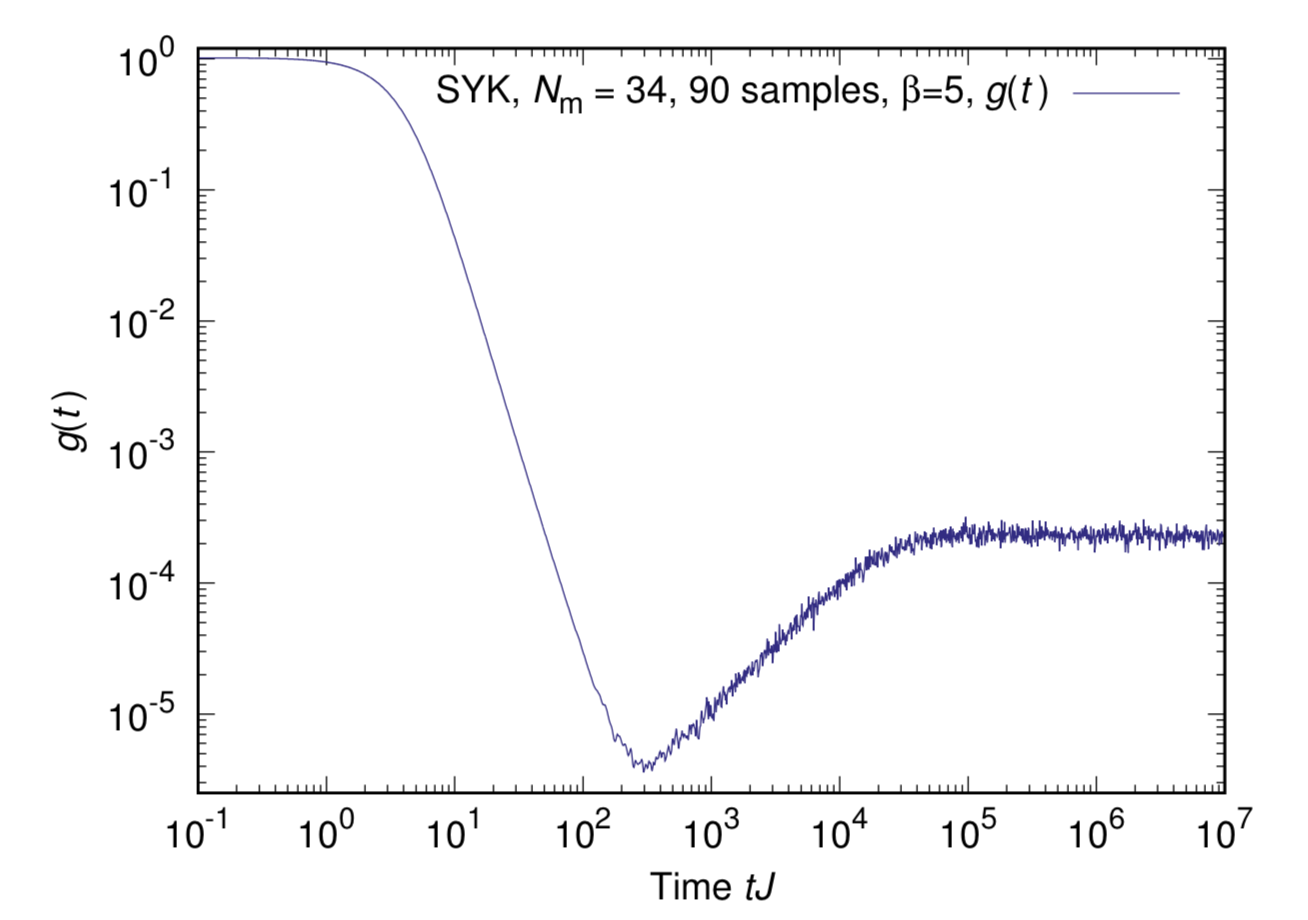
\includegraphics[width=10cm]{figures/spectralformfactor}
	\caption{SYK模型のスペクトラル形状因子。粒子数は34個であり、逆温度を$\beta = 5$としている。
		また$J_{ijkl}$のサンプルを90個用意した。
		ここでは横軸として時間に$J_{ijkl}$のスケール$J$を掛けて無次元化したものを用いた。
		最初は$g(t)$の値がゼロに落ちている。この領域をslopeと呼ぶ。
		その次には値が上昇している領域があり、この部分はrampと呼ぶ。
		rampは$t$に比例している。
		その後の水平な領域はplateauと呼ばれ、長時間平均を取った際に現れる値である。
		rampが終わってplateauに乗る時間をplateau時間$t_p$とする。
		この図は\cite{polchinski_chaos}より引用した。
	}
	\label{fig:spectralformfactor}
\end{figure}

$g(t)$はdisorder averageを取った量であり、ランダムカップリング$J_{ijkl}$についての揺らぎを
均したものであるため、図\ref{fig:spectralformfactor}のplateauには量子論で期待される大きい揺らぎ
が存在しない
\footnote{小さい揺らぎは見られるが、
	これは$J_{ijkl}$のサンプルを無限個にはできない事による数値計算上の理由である。}。
disorder averageを取らず、
1つの$J_{ijkl}$に対してのみプロットすると揺らぎが見られる\cite{polchinski_chaos}。

$g(t)$は3つの領域に区分される。
1つめは最初の値が降下している領域で、slopeと呼ばれる。
2つ目は降下が終わって上昇する領域で、rampという。rampは$t$に比例している。
ramp以降はplateauと呼ばれる領域が続く。plateauの高さが長時間平均である。

SYK模型やRMTの$g(t)$には共にrampやplateauの構造が見られる。
RMTにおける$g(t)$は具体的な解析が行われおり、特に行列のサイズのラージ極限での議論をこの後に述べる。
その後、それを踏まえてSYK模型に話を移す事にする。

\subsubsection{ランダム行列理論のスペクトラル形状因子}
\begin{figure}[ht]
	\centering
	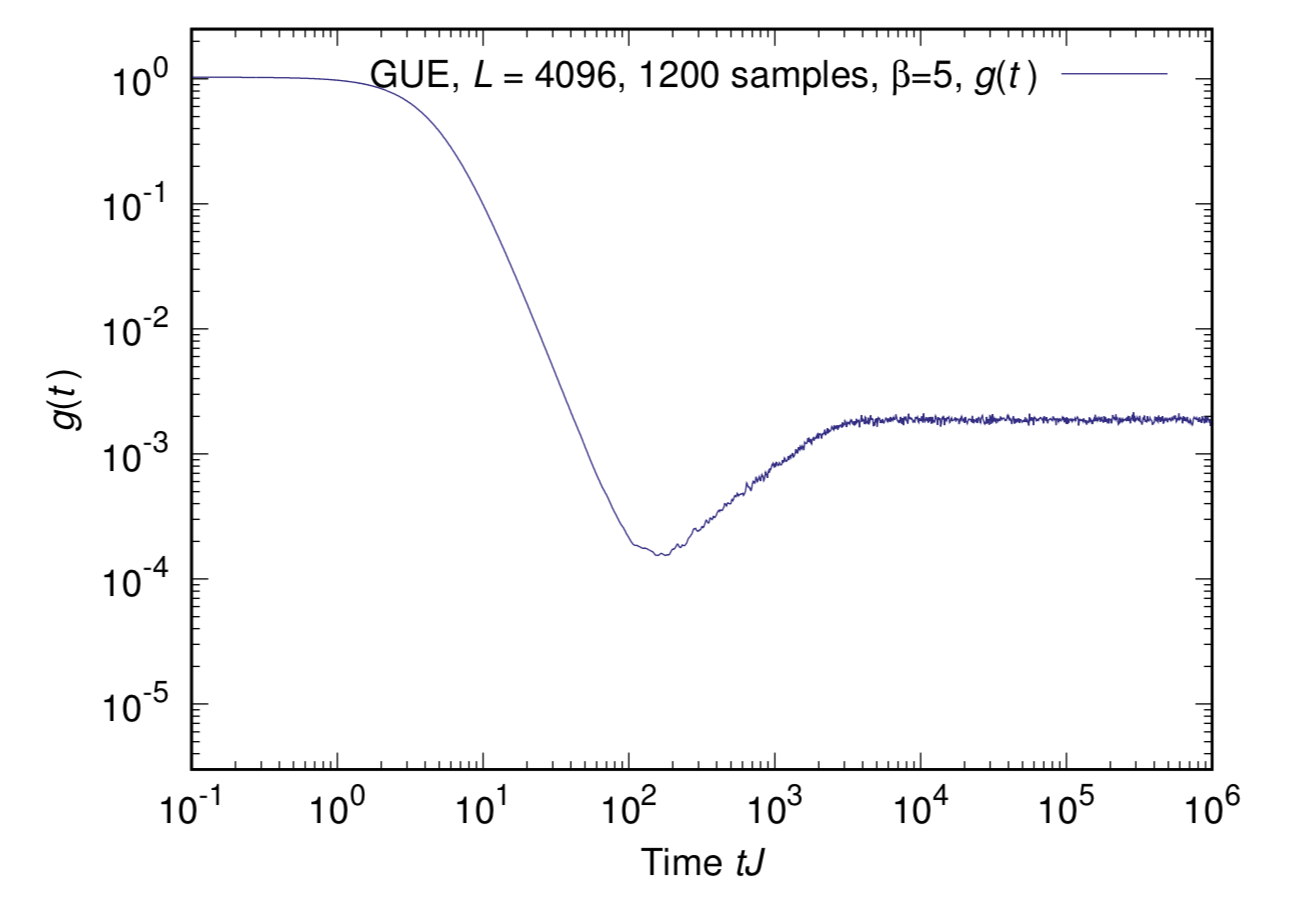
\includegraphics[width=10cm]{figures/spectralformfactor_inRMT}
	\caption{GUEにおけるスペクトラル形状因子。逆温度は$\beta=5$、行列のサイズは$L=4096$であり、
		サンプル数は1200個である。この図は\cite{polchinski_chaos}より引用した。
	}
	\label{fig:spectralformfactor_inRMT}
\end{figure}
ここではRMTの簡単なレビューを記述する。
特にランダム行列の持つ乱数の従う統計集団としてGUEを選ぶ。
この節の目標は図\ref{fig:spectralformfactor_inRMT}に表示されているGUEスペクトラル形状因子の、
slopeのlate-timeでの振る舞いやrampの初期の振る舞いを理解する事である。
結果は両方ともべき乗で表され、それを用いてslopeとrampが接続する時間を計算する。
なお、この時間をdip timeと呼ぶ。

階数$L$を持つエルミート行列$M$を考える。
これがGUEに属するとすると、統計平均は
\begin{align}
	\mathcal{Z}_{\mathrm{GUE}} = \int \prod_{i, j} dM_{ij}\ \exp\left(
		-\frac{L}{2}\tr\ M^2
	\right)
	\label{eq:GUEstatistics}
\end{align}
で与えられる。
エルミート行列$M$はSYK模型でのハミルトニアンに相当し、階数$L$はヒルベルト空間の次元に
対応する。
RMTとSYK模型の間の重要な違いの1つは摂動パラメータの違いである; SYK模型は$1/N$なのに対し、
RMTは$1/L \approx e^{-N}$である。

$M$の分配関数は
\begin{align}
	Z(\beta, t) = \tr\ e^{-\beta M - iMt}
	\label{eq:GUEpartition_function}
\end{align}
で定義される。
スペクトラル形状因子は\eqref{eq:spectral_form_factor}式と同様に定義される。
ただしdisorder average$\langle \cdot\rangle_J$は\eqref{eq:GUEstatistics}式によるGUEの
統計平均$\langle\cdot\rangle_{\mathrm{GUE}}$に置き換わる。

次にエルミート行列$M$を対角化し、基底をユニタリ変換する事を考える。
この変換により、固有値同士の"排斥力"を表すヤコビアンが現れる。
行列のサイズ$L$のラージ極限を取ると固有値分布はある密度$\rho$によって記述できる。
この$\rho$を物理的な密度として使い、$\tilde{\rho}$を規格化したものとする:
\begin{align}
	\int d\lambda\ \rho(\lambda) = L,\hspace{20pt}
	\int d\lambda\ \tilde{\rho}(\lambda) = 1,\hspace{20pt}
	\rho(\lambda) = L\tilde{\rho}(\lambda).
\end{align}
\eqref{eq:GUEstatistics}式において$M$のスペクトルを$\tilde{\rho}$として滑らかにすると、
GUEの統計平均は
\begin{align}
	\mathcal{Z}_{\mathrm{GUE}} = \int \mathcal{D}\tilde{\rho}(\lambda)\ e^{-S},
	\hspace{10pt}
	S 
	= -\frac{L^2}{2} \int d\lambda\ \tilde{\rho}(\lambda)\lambda^2
	+ L^2 \int d\lambda_1 d\lambda_2\ \tilde{\rho}(\lambda_1)\tilde{\rho}(\lambda_2)
		\log|\lambda_1 - \lambda_2|
\end{align}
と書き改められる。


\subsubsection{SYK模型のスペクトラル形状因子}

\subsection{スペクトラル形状因子の$G$、$\Sigma$による記述}

\pagebreak